% gold_memo.tex
%
% A seven-page research memo: financial gold flows and the US trade accounts.
% Four figures, declarative section headings, endnotes.
%
% Structure follows the brief, with two additions made after critiquing it:
%   - a closing recommendation section, because four diagnostic sections and no
%     prescription leaves the contribution unstated
%   - form conversion (400oz -> 100oz recasting) in section 3, which is the
%     structural fact most novel to a trade-statistics audience and which
%     explains why gross flows overstate net relocation
%
% NOT a Federal Reserve publication and deliberately not dressed as one.
%
% Build (two passes, for the endnote numbering):
%   pdflatex -interaction=nonstopmode gold_memo.tex
%   pdflatex -interaction=nonstopmode gold_memo.tex

\documentclass[11pt]{article}

\usepackage[letterpaper,margin=1.05in,top=1.0in,bottom=1.1in]{geometry}
\usepackage[T1]{fontenc}
\usepackage[utf8]{inputenc}
\usepackage{charter}
\usepackage[scaled=0.92]{helvet}
\usepackage{graphicx}
\usepackage{amsmath}
\usepackage{booktabs}
\usepackage{enumitem}
\usepackage{endnotes}
\usepackage{caption}
\usepackage{microtype}
\usepackage[hidelinks]{hyperref}
\usepackage{xcolor}

\definecolor{ink}{HTML}{121212}
\definecolor{soft}{HTML}{555555}
\definecolor{rule}{HTML}{BBBBBB}

\usepackage{titlesec}
\titleformat{\section}{\sffamily\bfseries\large\color{ink}}{}{0pt}{}
\titlespacing*{\section}{0pt}{14pt}{5pt}

\captionsetup[figure]{labelformat=empty, justification=raggedright,
  singlelinecheck=false, font={sf,small}, skip=6pt}

\setlength{\parskip}{6pt}
\setlength{\parindent}{0pt}
\renewcommand{\baselinestretch}{1.05}

\renewcommand{\enotesize}{\small}
\renewcommand\enoteheading{\section*{\sffamily\bfseries\large Notes}}

% \raggedright is needed because the figure environment centres everything,
% which left the notes block centred line by line.
\newcommand{\fignote}[2]{%
  \par\vspace{2pt}{\raggedright\sffamily\footnotesize\color{soft}%
  \textbf{Notes:} #1\par\textbf{Sources:} #2\par}}

\begin{document}
\pagestyle{empty}

% ------------------------------------------------------------------ masthead
{\sffamily\footnotesize\color{soft} ECONOMIC RESEARCH MEMO \hfill October 2026}

\vspace{4pt}
{\color{rule}\hrule height 2pt}
\vspace{10pt}

{\sffamily\bfseries\LARGE\color{ink}
Financial gold and the trade accounts:\\ why the ITA needs a bullion adjustment\par}

\vspace{6pt}
{\sffamily\small\color{soft} Samuel Moore\par}

\vspace{10pt}

% ------------------------------------------------------------------ abstract
{\sffamily\small\color{ink}
In the first quarter of 2025 the United States imported roughly 870 tonnes of
gold, more than twenty times what Americans buy as jewellery and retail
investment in a quarter. Within eleven months the metal had all gone back out.
This memo argues that these flows were financial rather than commercial, that
the gold market's structure is what makes them so, and that their passage
through the International Transactions Accounts left two official measures of
the U.S.\ goods balance pointing in opposite directions for three consecutive
quarters. Published GDP is unaffected; the national accounts already remove
nonmonetary gold. The monthly trade release does not --- and the adjustment
that fixes it is arithmetic on published data, verifiable against the national
accounts, and safe to apply as the occasion demands.\par}

\vspace{6pt}
{\color{rule}\hrule height 0.5pt}

% ====================================================================
\section{An outlier among traded goods}

Between November 2024 and March 2025 something unusual happened to one line of
the U.S.\ trade accounts. Gold imports, which had run between one and three
billion dollars a month for a decade, reached \$34.2 billion in January 2025
alone --- 10.5\% of all U.S.\ goods imports in a single month, from a commodity
that normally accounts for about one percent.

Then it reversed. Figure 1 places gold against the hundred most-traded U.S.\
commodity headings on the balance plane: exports on one axis, imports on the
other, averaged within three phases. Above the diagonal the United States is a
net importer of a good; below it, a net exporter. Most commodities barely move
between phases. Gold travels almost vertically upward into the surge, then down
and to the right into the reversal, ending as far below the diagonal as it
began above it. The right-hand panel shows the same excursion for the partner
that carried most of it: Switzerland.

\begin{figure}[htbp]
\centering
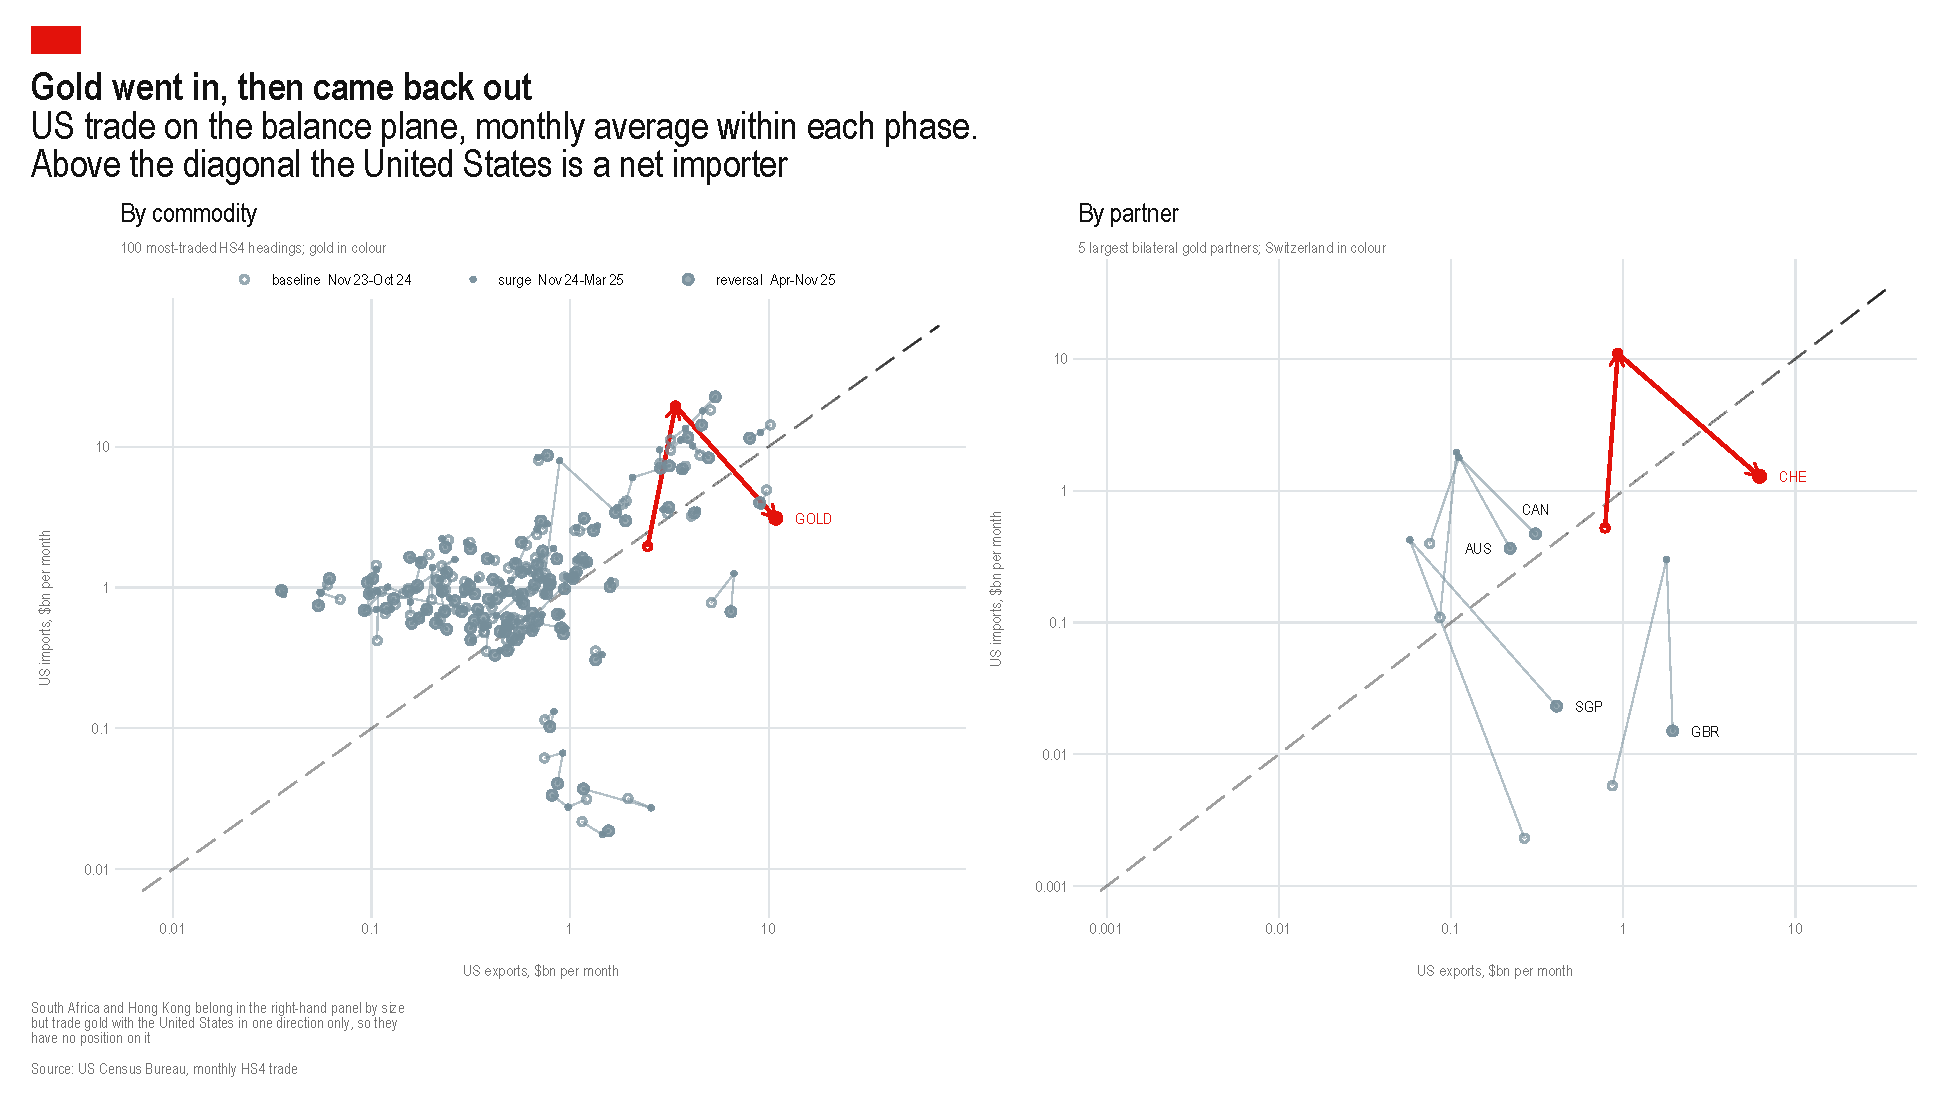
\includegraphics[width=\textwidth]{../figures/gold_panel.pdf}
\caption{\textbf{1. Gold's round trip, against every other traded good}}
\fignote{Monthly averages within each phase, log scales. Baseline is November
2023 to October 2024, surge November 2024 to March 2025, reversal April to
November 2025.}{U.S.\ Census Bureau, monthly HS4 trade.}
\end{figure}

The round trip is the first clue that this was not trade in the ordinary sense.
Cumulative net gold imports ran to \$80.0 billion by March 2025 and were back
through zero eleven months later, standing at \$47.6 billion \emph{negative} by
mid-2026: more metal left than had arrived. Across the whole period since 2015,
\$791 billion of gold crossed the U.S.\ border gross against a net of
\$-64 billion. Only 8\% of the metal that crossed stayed.

Goods that are bought get consumed, installed or worn. They do not come back.

% ====================================================================
\section{Nobody at either end wanted the metal}

A sceptical reader can still ask whether Americans were simply buying a lot of
gold. The answer is arithmetic, and Figure 2 gives it on both sides of the
account.

The upper panel sets U.S.\ gold imports against U.S.\ demand --- jewellery plus
bar and coin, which is every ounce Americans buy as ornament or hold as retail
investment. That benchmark is deliberately generous: bar and coin is investment
rather than fabrication, so including it makes the comparison harder to win.\endnote{Technology
demand --- electronics, dental, industrial --- would add little. It runs at
roughly 330 tonnes a year for the entire world, and the World Gold Council does
not publish it by country.} In 2025Q1 the United States imported 870 tonnes
against demand of 39 tonnes: twenty-two times a quarter's consumption, in one
quarter. U.S.\ demand averages 53 tonnes a quarter over this window and has
never exceeded 75.

\begin{figure}[htbp]
\centering
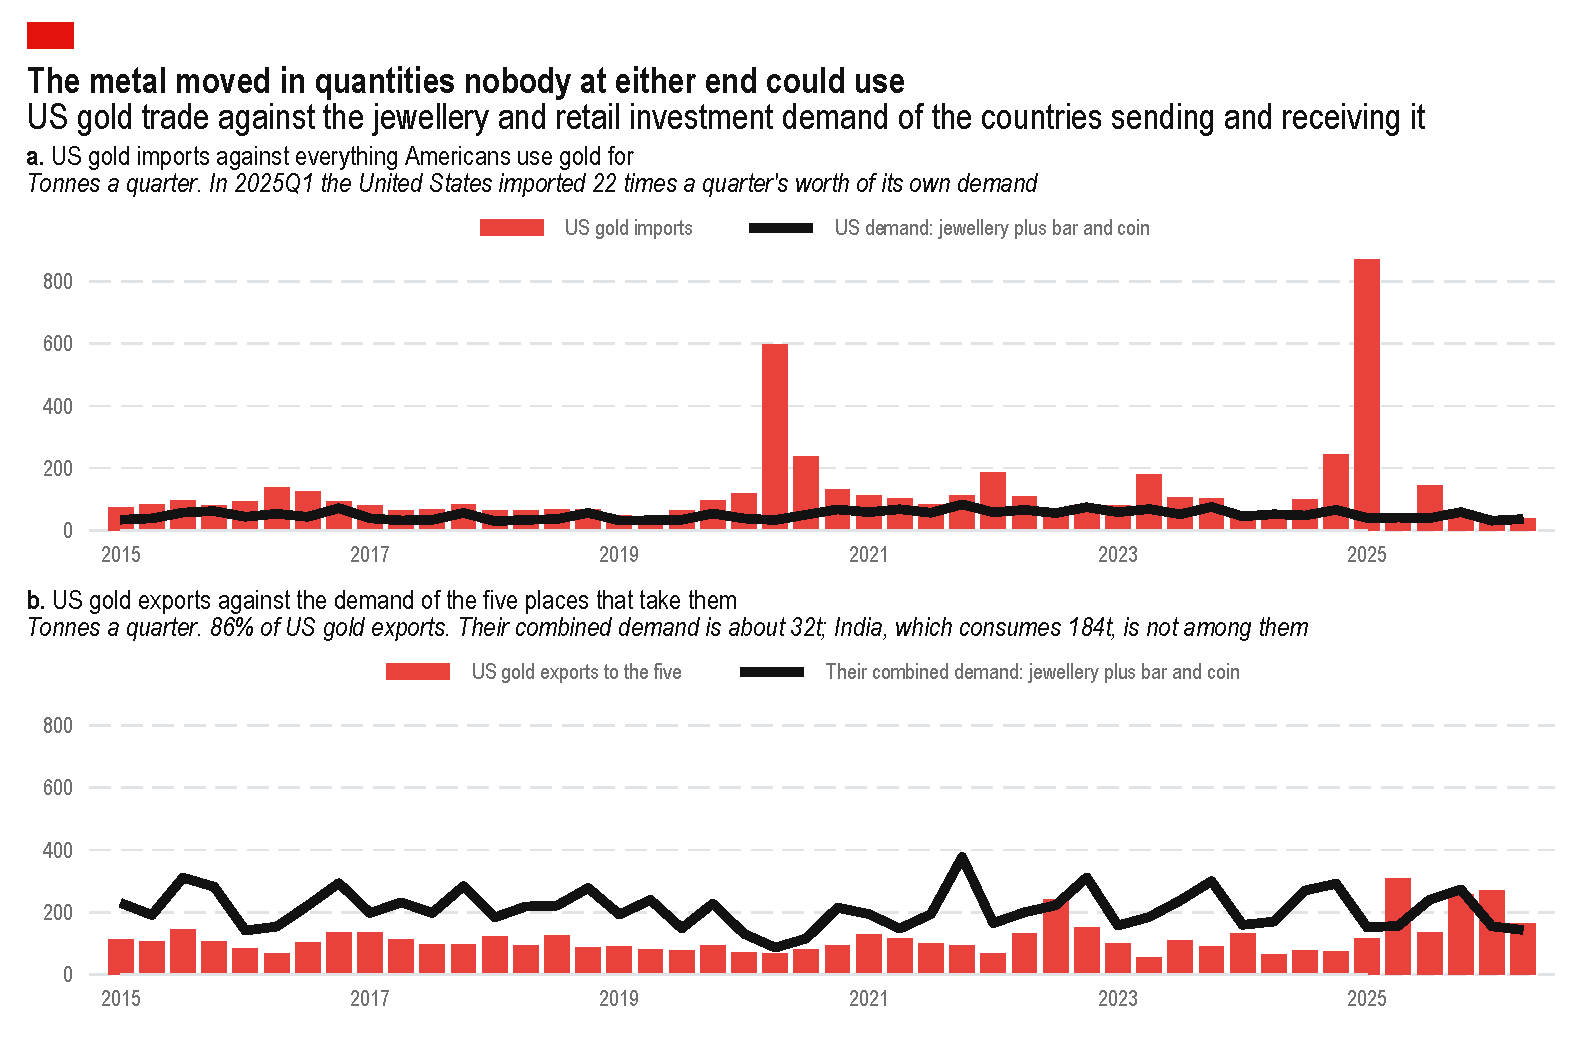
\includegraphics[width=\textwidth]{../figures/flows_vs_fabrication.pdf}
\caption{\textbf{2. The flows against what the metal is actually used for}}
\fignote{Tonnes a quarter, converted from Census dollar values at the LBMA PM
monthly average and 32,150.7 troy ounces to the tonne. Demand is jewellery plus
bar and coin. The five destinations are chosen from the trade data, not
assumed. The World Gold Council does not break out Swiss jewellery demand, which
sits inside a regional aggregate, so Switzerland contributes bar and coin only
and the partner benchmark is marginally understated.}{U.S.\ Census Bureau; World
Gold Council, \textit{Gold Demand Trends}; LBMA.}
\end{figure}

The lower panel does the same for exports, against the demand of the five
destinations that take them. Those five --- Canada, Hong Kong, Singapore,
Switzerland and the United Kingdom --- account for 86.6\% of U.S.\ gold exports
to identified countries. Their \emph{combined} gold demand is about 32 tonnes a
quarter. Peak quarterly exports to them were 327 tonnes.

The composition is sharper than the ratio. India consumes 184 tonnes a quarter,
more than those five put together, and is not among the destinations at all.
The United States ships its gold to the five places that barely use any, and
not to the one place that uses more than all of them combined. What the five do
have in common is infrastructure: Switzerland refines, and London, Hong Kong
and Singapore vault.

So something moved 870 tonnes of metal that nobody at either end had any use
for, and then moved most of it back. What?

% ====================================================================
\section{Two prices for the same metal}

Gold trades in two places that are not quite the same market. London is an
over-the-counter market in 400-ounce \textit{Good Delivery} bars, held
unallocated in vaults and settled by book entry. New York is a futures exchange,
COMEX, whose contract delivers 100-ounce bars into registered exchange
warehouses.\endnote{A futures contract is a standardised agreement to deliver a
commodity at a stated future date; its settlement price is the exchange's
official daily mark. Warehouse stocks are reported in two categories,
\textit{registered} (available to settle contracts) and \textit{eligible}
(stored but not pledged).} The metal is identical. The venue, the bar, and the
legal form of the claim are not.

Because the two can be converted into each other, arbitrage ties their prices
together --- but only loosely, and the slack is the subject of Figure 3. The
futures price should exceed the spot price by the cost of carrying metal to
delivery: financing plus storage. That is the same no-arbitrage logic as covered
interest parity, with storage cost in place of a foreign interest rate. Our
estimate of the New York premium strips out the carry and expresses what remains
at a constant ninety-day horizon.\endnote{The premium is the intercept of a
daily open-interest-weighted projection of the whole futures curve onto
days-to-delivery, less London spot, corrected for the three-and-a-half hours
between the COMEX settlement and the London benchmark. Regressing on the raw
dollar spread would confound the dislocation with the delivery calendar: at 4.5\%
financing on \$4,400 gold, the roll alone generates a sawtooth of about \$33 an
ounce.}

\begin{figure}[htbp]
\centering
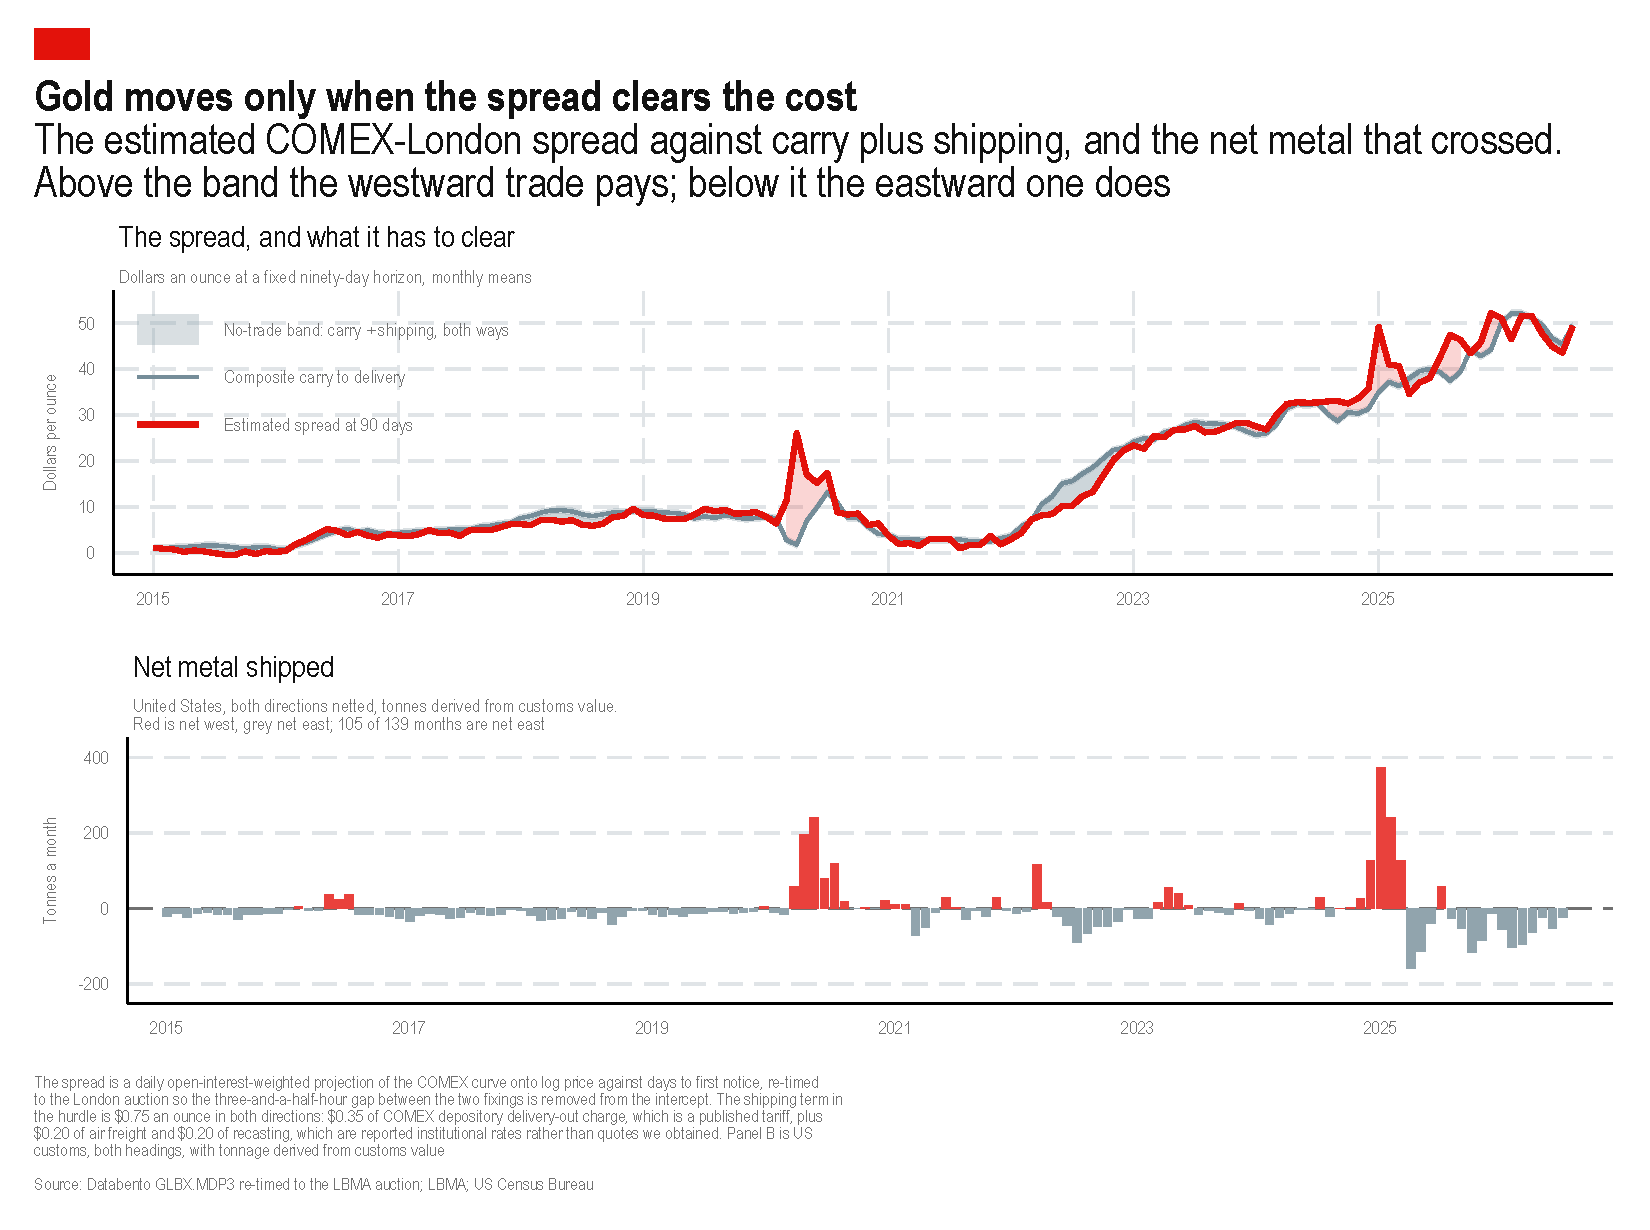
\includegraphics[width=0.96\textwidth]{../figures/spread_vs_hurdle.pdf}
\caption{\textbf{3. The COMEX--London spread against what it has to clear}}
\fignote{The hurdle is carry plus an all-in transfer cost of \$0.75 an ounce:
freight and insurance, recasting, and the exchange's delivery-out charge.
Arbitrage pays only when the spread clears it.}{CME via Databento; LBMA; U.S.\
Census Bureau.}
\end{figure}

Metal does not move whenever the two prices differ. It moves when the
difference exceeds the cost of moving it --- freight and insurance, the
exchange's delivery-out charge, and recasting. We put that hurdle at about
\$0.75 an ounce.\endnote{Roughly \$0.20 freight and insurance, \$0.20
recasting, and \$0.35 for delivery out of a CME-approved depository. The
relationship is therefore kinked, not linear: below the hurdle nothing moves.}
The relationship is a threshold, not a slope, and Figure 3 shows the spread
clearing that threshold in late 2024 and the metal following.

One further feature of the market matters for what the trade statistics
record. London bars and COMEX bars are different sizes, so relocating metal
between the two generally requires recasting, and the refining capacity sits
mostly in Switzerland. A single tonne relocated from London to New York can
therefore be recorded as several separate crossings --- out of the United
Kingdom, into Switzerland, out of Switzerland, into the United States. The
gross trade footprint of a relocation substantially exceeds the relocation
itself. This is why Switzerland dominates the partner panel of Figure 1, and
why the 2025 episode was cheap in real resources: we estimate the whole
operation cost on the order of \$243 million in freight, insurance, recasting
and transit financing, about 0.14\% of the value shuttled.

% ====================================================================
\section{What it did to the trade accounts}

The Bureau of Economic Analysis publishes the U.S.\ goods balance twice. The
International Transactions Accounts, which underlie the monthly trade release,
count nonmonetary gold as a good --- correctly, under the international
standard.\endnote{BPM6 classifies nonmonetary gold as a good and monetary gold
as a financial asset. The ITA treatment is not an error.} The national accounts
remove it outright, replacing it with domestic production less industrial use.
In ordinary times the two barely differ and no one needs to know which they are
reading.

\begin{figure}[htbp]
\centering
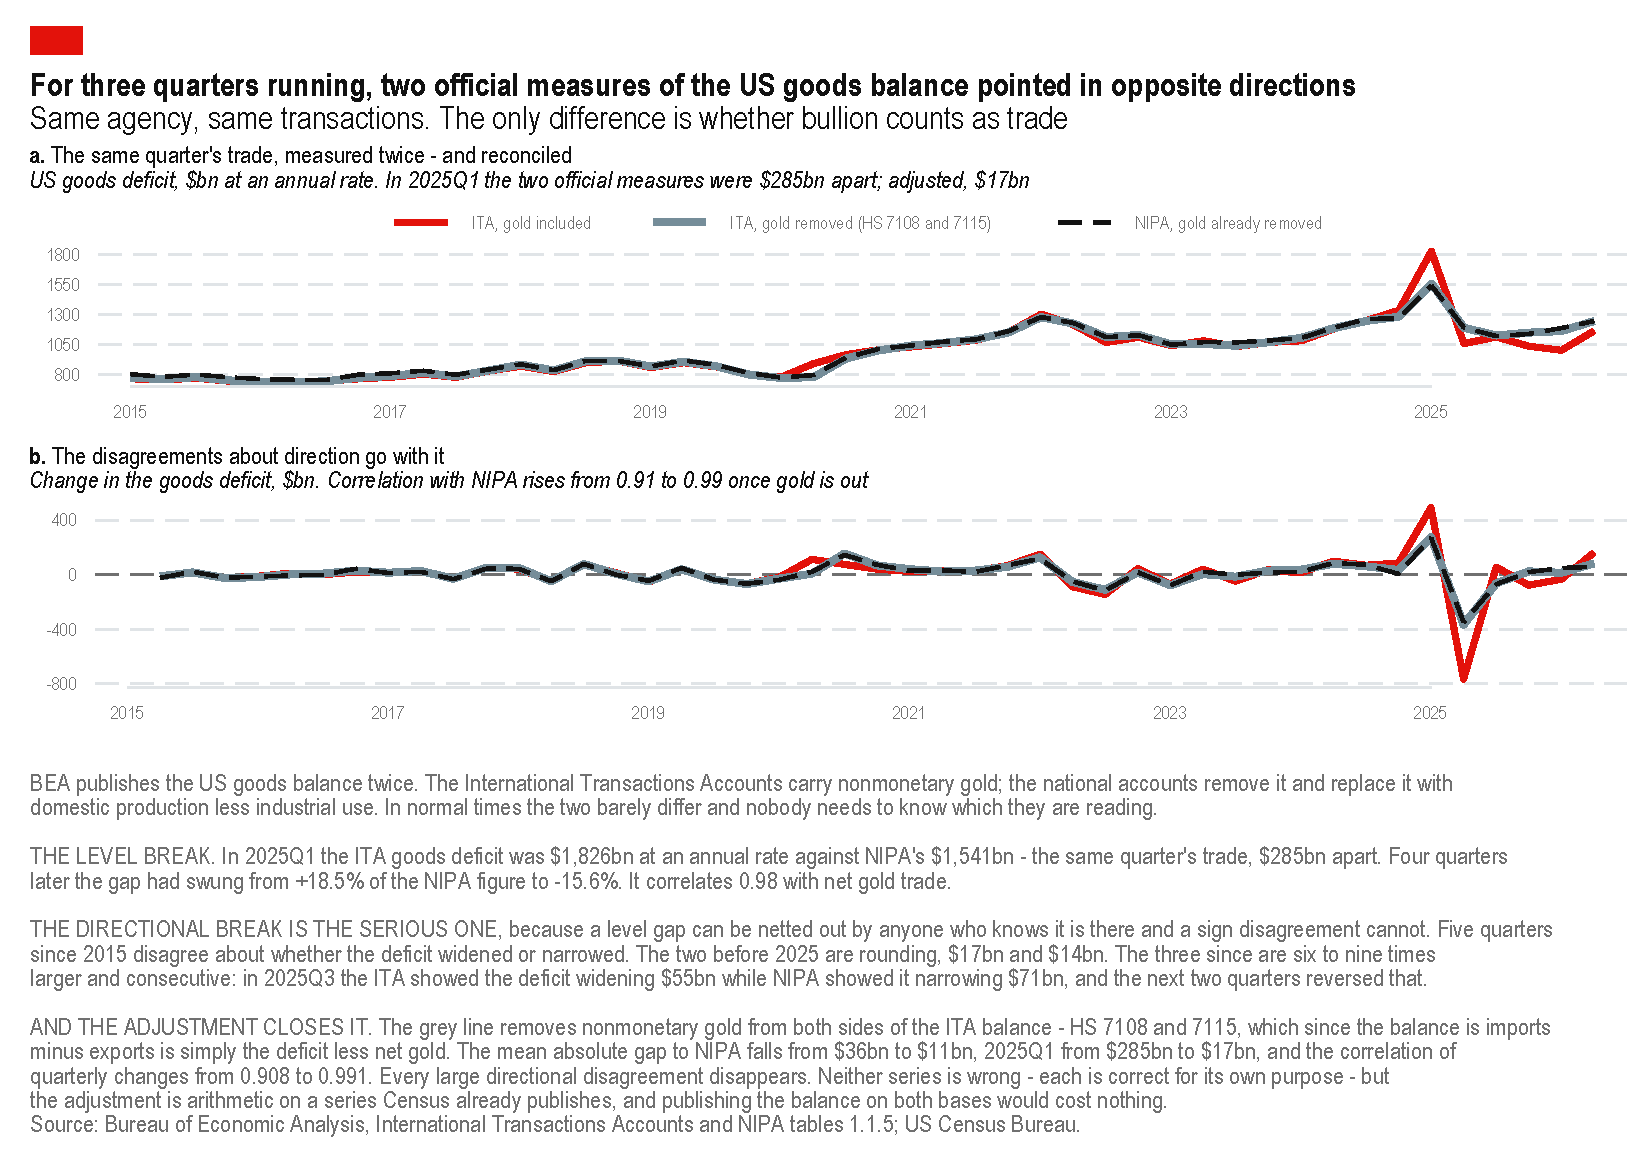
\includegraphics[width=\textwidth]{../figures/ita_nipa_comparability.pdf}
\caption{\textbf{4. The same quarter's trade, measured twice}}
\fignote{Quarterly, at annual rates. The adjusted series removes nonmonetary
gold (HS 7108 and 7115) from both sides of the ITA balance, which because the
balance is imports less exports is the deficit less net gold.}{Bureau of
Economic Analysis, International Transactions Accounts and NIPA table 1.1.5;
U.S.\ Census Bureau.}
\end{figure}

In 2025Q1 they differed by \$285 billion at an annual rate --- the ITA goods
deficit at \$1,826 billion against the national accounts' \$1,541 billion, a
gap of 18.5\% of the latter. Four quarters later the gap had swung to
\textit{minus} 15.6\%. Across the window it correlates 0.99 with net gold
trade.

A level gap can be netted out by anyone who knows it is there. A disagreement
about direction cannot, and that is what happened next. In the twenty-five
quarterly changes since 2020 the two measures disagree about whether the
deficit widened or narrowed exactly three times --- and all three are
consecutive. In 2025Q3 the trade release showed the deficit widening by \$55
billion while the national accounts showed it narrowing by \$71 billion; the
next two quarters reversed that. For three quarters running, one official U.S.\
measure of the external position said it was improving while the other said it
was deteriorating.

The claim is not that either series is wrong. Each treatment is correct for its
own purpose. The claim is that a correct series stopped being informative about
what its readers use it for, and did so without warning them.

% ====================================================================
\section{Adjust it yourself, and check your work}

The practical conclusion is a modest one: when gold is moving, take it out of
the monthly trade balance before reading anything into the number. The
adjustment is arithmetic, the inputs are published, and --- unusually for an
ad-hoc correction --- you can verify that you have done it right.

The arithmetic is one line. Because the balance is imports less exports, taking
nonmonetary gold out of both sides is the same as subtracting net gold:
\[
  \text{balance}^{\text{adj}}_{t}
  \;=\;
  \text{balance}_{t} - \bigl(\text{gold imports}_{t} - \text{gold exports}_{t}\bigr).
\]
Both terms come from the Census monthly HS series, under headings 7108 and
7115.\endnote{HS 7108 is unwrought and semi-manufactured gold; 7115 covers
articles of precious metal, under which a large share of the 2025 bar inflow
was entered. Using 7108 alone would miss most of the episode.}

What makes this safe rather than merely convenient is that it can be checked.
Figure 4's third line is exactly that calculation, and it lands on the national
accounts: the mean absolute gap falls from \$48 billion to \$9 billion, the
2025Q1 discrepancy from \$285 billion to \$17 billion, the correlation of
quarterly changes rises from 0.918 to 0.992, and all three directional
disagreements vanish. The adjusted series does not merely look tidier --- it
reproduces an independently constructed official aggregate that was built to a
different standard by a different part of the same agency. An ad-hoc
correction with an external benchmark is not really ad hoc; it is a replication.

A reasonable trigger is gold's share of goods trade. Below about one percent,
which is where it sat for most of the decade before 2020, the adjustment
changes nothing and can be ignored. Above a few percent it is worth making, and
in months like January 2025, when gold reached 10.5\% of goods imports, reading
the headline without it is reading mostly bullion.

The agencies could make this easier by publishing the goods balance on both
bases --- as reported, and excluding nonmonetary gold. The underlying series
are already collected and the adjustment is already computed for the national
accounts, so the cost is close to zero. But nobody needs to wait for that. The
data to do it is published every month.

Gold will do this again. The structure that produced the 2025 episode is
permanent: two venues, two bar standards, a transfer cost small enough that any
material dislocation pays for moving metal, and a stock of above-ground bullion
large enough that the quantities which clear it dwarf anything the metal is
used for. The next dislocation will move the same kind of volume through the
same accounts. Readers who understand why the metal moves, and who adjust for
it when it does, will not be misled by the headline.

\clearpage
\theendnotes

\end{document}
